\section{Related Work}
This section discusses the related works about early detection of forest disturbance and the big data systems that support it. The topic requires time series modeling and spectral analysis and unsupervised learning and large-scale geospatial data management. Research studies differ from each other because they use different assumptions and data requirements and scalability requirements.

Satellite imagery has become an essential data source for monitoring forest conditions over large regions. Modern sensors such as Sentinel-2 and Landsat create continuous time series data which contains multi-spectral information that detects physiological stress before humans can understand it through visual inspection. The datasets present three major obstacles which stem from their size and frequency and spatial distribution because they require big-data management solutions. Long-term monitoring at regional or continental scales requires systems that enable effective storage and indexing and distributed processing capabilities. A brief comparison of how these research categories address these challenges is shown below:


\begin{table*}[t]
  \centering
  \caption{Comparison of Change Detection and Distributed Framework Methods}
  \label{tab:method-comparison}
  \small
  \begin{tabularx}{\textwidth}{@{} >{\hsize=1.0\hsize\RaggedRight}X >{\hsize=1.2\hsize\RaggedRight}X >{\hsize=0.8\hsize\RaggedRight}X >{\hsize=1.0\hsize\RaggedRight}X @{}}
    \toprule
    \textbf{Category} & \textbf{Main Idea} & \textbf{Unit of analysis} & \textbf{Limitations} \\ 
    \midrule
    Statistical Time-Series Modeling\cite{bfast, nrt-anomalies} & Work around seasonal pattern & Per-pixel of image & Require large historical baseline \\ \addlinespace
    Spectral \& Species-Specific   \cite{ts-sentinel,jamali2024, bark-beetle} & Tailored method based on forest type or tree species & Multi-index, Sentinel-2 & Can lead to overfitting in a specific region. Unable to give a general model\\ \addlinespace
    Unsupervised Learning  \cite{ndvi, dl-forest, Zhang25082025, Prithvi-100M-preprint} & Pre-training on massive unlabeled data to understand `normal' behavior before fine-tuning for specific tasks &  band sequences; NDVI index trends & Requires repeated access to large datasets \\ \addlinespace
    Geospatial Big-Data Systems \cite{rdpro, icde-geospatial} & Distributed storage, indexing, and raster processing & Full space $\times$ time archives & Strong scalability and I/O guarantees \\ 
    \bottomrule
   \end{tabularx}
\end{table*}

% removed  Learning healthy pattern and than finding anomaly

\subsection{Statistical Time-Series Modeling}
\begin{wrapfigure}{r}{0.5\textwidth}
    \centering
    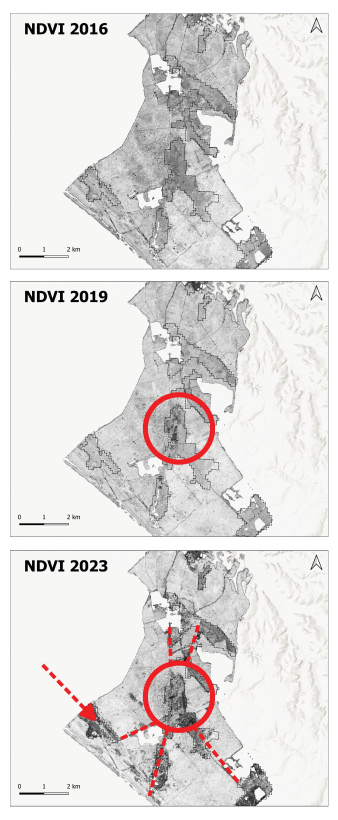
\includegraphics[width=0.25\textwidth]{figures/ndvi.png}
    \caption{Temporal sequence of the NDVI maps computed as annual average from GEE for the Castel Porziano area from \cite{ndvi}}
    \label{fig:ndvi}
\end{wrapfigure}
% These approaches are simple and interpretable. They work well for large areas but depend on efficient access to long pixel histories  a challenge addressed by scalable geospatial systems like \cite{rdpro, isprs-cube}.

Vegetation indices such as the \textit{Normalized Difference Vegetation Index} (NDVI) collected over years from platforms such as \textit{Sentinel-2} and \textit{Landsat} are widely used to quantify vegetation condition from optical satellite imagery and have served as a proxy for canopy greenness and structural health. Lasaponara et al.\ \cite{ndvi} demonstrate how dense Sentinel-2 NDVI records can be segmented into stable periods and change points using a continuous monitoring framework. By identifying moments when the time series departs from its expected seasonal behavior and fitting trend models to those segments, their approach captures both the timing and magnitude of vegetation stress linked to pest activity. Likewise, Zhang et al.\ \cite{forests-survey} construct a seasonal model of NDVI patterns and then monitor departures from this expected curve using an adaptive statistical monitoring approach that emphasizes persistent deviations rather than short-term noise. Their method detects both sudden disturbances, such as fire or harvest, and gradual canopy decline caused by insect damage or degradation.


The BFAST model \cite{bfast} decomposes vegetation-index time series into trend, seasonal, and remainder components and identifies structural breaks that may indicate disturbance. This is useful for forests because seasonal cycles often hide early stress signals.
A near-real-time anomaly framework \cite{nrt-anomalies} was also proposed which builds long-term baselines for vegetation indices and converts deviations into standardized anomaly scores. The method uses a small set of greenness and moisture indices and aims to work across different forest types.

Together, these studies show that vegetation stress can be identified by first establishing a historical seasonal baseline and then systematically monitoring departures from that baseline over time (see Figure \ref{fig:ndvi}). 

\subsection{Spectral and Species-Specific}

Some studies argue that generic vegetation indices are not sufficient because different forest species exhibit stress responses in different spectral regions and at different temporal scales. Rather than relying solely on generalized NDVI-based thresholds, spectral and species-specific approaches incorporate domain knowledge about vegetation physiology to improve early detection sensitivity.

A kernel-based early detection framework for bark beetle infestation uses dense Sentinel-2 vegetation index time series and integrates temporal behavior with local spatial context to generate anomaly scores \cite{jamali2024}. By modeling subtle deviations in spectral trajectories, the method is able to identify early infestation signals prior to visible crown discoloration. Unlike purely structural break point approaches, kernel-based models capture gradual, low-magnitude spectral shifts that characterize early-stage stress.

Carletti et al~\cite{ts-sentinel} further demonstrate that species-specific spectral responses must be considered when designing detection frameworks. Their analysis of Sentinel-2 time series across conifer species shows that red-edge and water-sensitive indices behave differently depending on tree species and environmental conditions. They also emphasize that longer temporal windows are often required to stabilize early-warning indicators and reduce noise from seasonal variability.

Similarly, König et al~\cite{bark-beetle} find that Sentinel-2 red-edge (CRE) and SWIR-based (NBR) indices achieve higher spatial accuracy in spruce forests by targeting chlorophyll and moisture loss. Their results suggest that spectral sensitivity to specific physiological traits is more vital for early detection than increased temporal density from multi-sensor fusion. Conversely, they highlight the inadequacy of C-band SAR for identifying the low-magnitude structural shifts present in early infestations.

Together, these studies highlight a key trade-off: species-aware spectral modeling improves detection precision but may limit generalizability across heterogeneous forest types. Moreover, such approaches require access to dense multi-temporal raster archives to analyze long pixel histories efficiently, motivating scalable storage and indexing mechanisms such as the space-time cube model \cite{isprs-cube}.

\subsection{Unsupervised Learning}

Another line of research moves beyond explicit statistical modeling and allows systems to learn ``normal'' vegetation behavior directly from historical data. Unsupervised deep learning approaches, particularly sequence-based architectures, analyze multi-spectral time-series signals to capture temporal dependencies that may not be fully represented by predefined trend or seasonal components.

An LSTM autoencoder trained on healthy spruce stands learns typical Sentinel-2 spectral sequences and identifies potential disturbances through reconstruction error when incoming observations deviate from learned patterns \cite{dl-forest}. Because the model encodes temporal dynamics rather than relying on explicit break detection, it can identify gradual or nonlinear stress patterns that may not produce clear structural breakpoints detectable by classical time-series decomposition methods such as BFAST \cite{bfast}. In several cases, disturbances were detected weeks before visible canopy symptoms emerged.

As an alternative to reconstruction, recent frameworks~\cite{Zhang25082025} have adopted Self-Supervised Learning (SSL) architectures to distill robust forest health representations directly from unlabeled imagery. These models typically employ Transformer-based encoders to identify significant land-cover transitions by learning temporal invariants across massive multi-sensor archives. By prioritizing high-level feature extraction over simple pixel-wise reconstruction, these architectures effectively isolate low-magnitude vegetation anomalies from natural seasonal variance without requiring pre-defined change points or manual masks.

Expanding on feature-based methods, the Prithvi-100M foundation model~\cite{Prithvi-100M-preprint} utilizes a SSL framework to address the label scarcity bottleneck. They pre-train the model on massive unlabeled multispectral imagery, using a Masked Autoencoder (MAE). During this stage, the encoder learns to reconstruct the original signal from visible patches, enabling the model to distill generalized geospatial representations across space and time. Following this pre-training, the model undergoes supervised fine-tuning for specific downstream tasks, such as flood mapping or wildfire scar segmentation, using significantly smaller labeled datasets. 

Overall, unsupervised learning methods complement statistical approaches rather than replacing them. Statistical models provide interpretability and explicit change-point identification, whereas deep learning models offer flexibility in capturing complex temporal patterns. Supporting both paradigms at scale requires distributed processing frameworks capable of efficiently managing large spatiotemporal raster archives.

\subsection{Geospatial Big-Data Systems and Monitoring Pipelines}
A recent study in Madagascar compared seven global satellite data products and found substantial disagreement in forest change detection, particularly in drier ecoregions \cite{worldcover}. This highlights the challenges of applying global models to local contexts and underscores the need for harmonized, adaptable systems like RDPro \cite{rdpro}.

To address such challenges, scalable data models and processing frameworks have been proposed. The space-time cube model organizes raster time series into a multidimensional structure indexed along the temporal axis \cite{isprs-cube}. It enables fast retrieval of pixel histories and supports early detection pipelines that repeatedly query long time series for millions of pixels. Figure \ref{fig:accuracy}, adapted from ISPRS IJGI \cite{isprs-cube}, illustrates how this model validates GLAD forest cover data using National Forest Inventory (NFI) and CEH habitat layers, highlighting commission and omission errors across habitat types and canopy densities.

\begin{figure}[h]
    \centering
    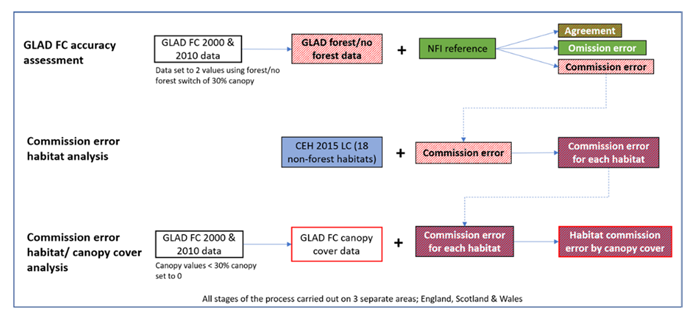
\includegraphics[width=\linewidth]{figures/accuracy_assessment.png}
    \caption{Accuracy Assessment Pipeline for GLAD Forest Cover. Adapted from ISPRS IJGI \cite{isprs-cube}, this flowchart illustrates the multi-step process used to assess the accuracy of GLAD forest cover data using NFI reference datasets and CEH habitat layers. It includes forest/no-forest classification, commission and omission error analysis, and habitat-based validation.}
    \label{fig:accuracy}
\end{figure}

Complementing this, RDPro introduces the "Maplet" model, which partitions large raster datasets into small tiles for direct, distributed processing \cite{rdpro}. This reduces data movement and supports repeated vegetation index computations in forest-monitoring workflows. The ICDE 2019 study further enhances these systems by proposing optimized storage layouts and spatiotemporal indexing strategies that improve data locality and I/O performance \cite{icde-geospatial}.

Unlike data-organization approaches such as the space-time cube, which primarily optimize indexing and historical retrieval, distributed frameworks like RDPro and Apache Sedona emphasize scalable execution and parallel processing. Together, these approaches demonstrate that both efficient data layout and distributed computation are necessary to support large-scale vegetation monitoring workflows.



At the application level, environmental monitoring pipelines integrate these infrastructure components to deliver operational insights. A study in \textit{Science of the Total Environment} uses large-scale disturbance alerts to examine how vegetation anomalies relate to climate and land-use pressures \cite{worldcover}. Similarly, the Digital Earth pipeline combines multi-sensor inputs, time-series models, and distributed infrastructure to support near-real-time forest disturbance alerts at continental scales \cite{bark-beetle}.

Together, these system-level contributions form the operational backbone for early detection pipelines by addressing the complementary challenges of data organization, scalable processing, and efficient retrieval of long-term spatiotemporal archives required for responsive forest monitoring.
